\documentclass[11pt, titlepage]{article}
% Common packages/environments to remove clutter

% Packages
\usepackage[utf8]{inputenc}
\usepackage{amsmath, amsfonts, amssymb, amsthm, enumitem, tikz, import, mathtools}
\usepackage[
  top=2cm,
  bottom=2cm,
  left=3cm,
  right=3cm,
  headheight=17pt,
  includehead, includefoot,
  heightrounded,
]{geometry}

% Problem environment
\newtheoremstyle{emptyplain}
    {}          % default space above
    {}          % default space below
    {}          % default body font
    {}          % no indent
    {\bfseries} % head font
    {.}         % punctuation after theorem head
    { }         % space after theorem head
    {#3}
\theoremstyle{emptyplain}
\newtheorem*{problem}{}

% Solution Environment
\newenvironment{solution}{
  \begin{proof}[Solution]
    \vspace{-2px}
    \setlength{\parskip}{4px}
    \setlength{\parindent}{0px}
}{
\end{proof}
}

\usepackage{gensymb}

% Opening
\title{Math 2552 Written HW Set 2}
\author{Akash Narayanan}
\date{February 2, 2021}

\begin{document}
  \maketitle

  % Judson 1.3 #21
  \begin{problem}[Judson 1.3.21]
    Consider the differential equation \(y' = f(y)\), where the graph of \(f(y)\) is given below.
    Draw the phase line for the equation and classify each equilibrium solution as a sink, a source, or a node.
    \begin{figure}[h]
      \centering
      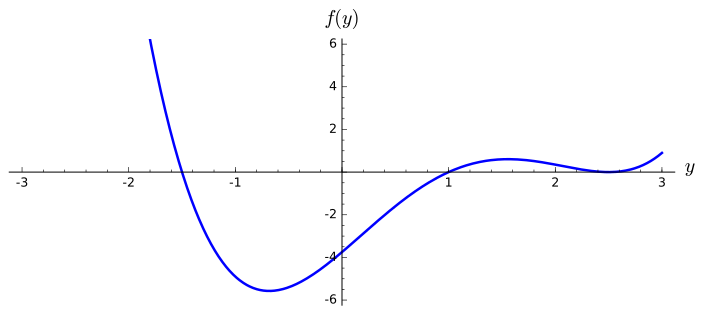
\includegraphics[scale=0.5]{media/Graph 1-3-21.png}
    \end{figure}
  \end{problem}

  \begin{solution}
    The equilibrium solutions are those points where \(f(y) = 0\).
    This occurs at \(y = -1.5\), \(y = 1\), and \(y = 2.5\).
    We can classify the equilibrium solutions by evaluating the derivative at various values of \(y\) as shown in the table below.
    \begin{center}
      \begin{tabular}{ |c|c| }
        \hline
        \(y\) & \(y\) \\
        \hline
        \(y < -1.5\) & \(y' > 0\) \\
        \hline
        \(-1.5 < y < 1\) & \(y' < 0\) \\
        \hline
        \(1 < y < 2.5\) & \(y' > 0\) \\
        \hline
        \(2.5 < y\) & \(y' > 0\) \\
        \hline
      \end{tabular}
    \end{center}
    Using the table, we can draw the corresponding phase diagram.

    \begin{figure}[h]
      \centering
      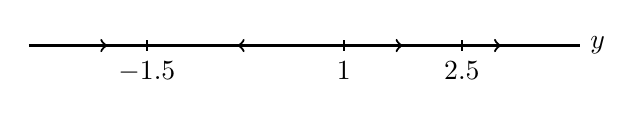
\begin{tikzpicture}[thick]
        \foreach \X in {-1.5, 1, 2.5} {
          \draw (\X, 2pt) -- (\X, -2pt) node [below] {\(\X\)};
        }
        \foreach \X in {-2, 1.75, 3} {
          \draw [->] (\X - 0.1, 0) -- (\X, 0);
        }
        \foreach \X in {-0.25} {
          \draw [<-] (\X - 0.1, 0) -- (\X, 0);
        }
        \draw (-3, 0) -- (4, 0) node [right] {\(y\)};
      \end{tikzpicture}
    \end{figure}
    From here, it becomes clear that \(y = -1.5\) is a \textbf{sink}, \(y = 1\) is a \textbf{source}, and \(y = 2.5\) is \textbf{stable}.
  \end{solution}

  \pagebreak

  % Trench 2.3 #7
  \begin{problem}[Trench 2.3.7]
    Find all \((x_{0}, y_{0})\) for which the initial value problem
    \begin{equation*}
      y' = \ln(1 + x^{2} + y^{2}), \; y(x_{0}) = y_{0}
    \end{equation*}
    has \textbf{(a)} a solution \textbf{(b)} a unique solution on some open interval that contains \(x_{0}\).
  \end{problem}

  \begin{solution}
    The Existence and Uniqueness Theorem states that the initial value problem has at least one solution if
    \(f(x, y) = \ln(1 + x^{2} + y^{2})\) is continuous on an open rectangle
    \begin{equation*}
      R : \{a < x < b, c < y < d\}
    \end{equation*}
    containing \((x_{0}, y_{0})\).
    Furthermore, if both \(f\) and \(f_{y}\) are continuous on \(R\), then the initial value problem has a unique solution on an open subinterval of \((a, b)\) containing \(x_{0}\).

    \(f(x, y)\) is continuous for \(1 + x^{2} + y^{2} > 0\). Since \(x^{2} + y^{2} > 0\) for all \((x, y)\), \textbf{(a)} the initial value problem has at least one solution for all \((x_{0}, y_{0})\).

    For \textbf{(b)}, we calculate
    \begin{equation*}
      f_{y}(x, y) = \frac{2y}{1 + x^{2} + y^{2}}
    \end{equation*}
    Rational functions are only discontinuous at points where the denominator is 0, but \(1 + x^{2} + y^{2}\) is greater than 0 for all \(x\) and \(y\).
    Since \(f_{y}(x, y)\) is continuous at all \((x, y)\), the Existence and Uniqueness Theorem guarantees that the initial value problem has a unique solution for all \((x_{0}, y_{0})\).
  \end{solution}

  \pagebreak

  % Trench 4.2 #5
  \begin{problem}[Trench 4.2.5]
    An object with initial temperature 150\degree C is placed outside, where the temperature is 35\degree C.
    Its temperature at 12:15 and 12:20 are 120\degree C and 90\degree C, respectively.
    \begin{enumerate}
      \item At what time was the object placed outside?
      \item When will its temperature be 40\degree C?
    \end{enumerate}
  \end{problem}

  \begin{solution}
    By Newton's Law of Cooling, the temperature of the object \(T(t)\) may be modeled with the following differential equation and initial value:
    \begin{equation*}
      \frac{dT}{dt} = k (T - 35), \; T(0) = 150
    \end{equation*}
    This is a separable equation which we can solve as follows:
    \begin{gather*}
      \int \frac{dT}{T - 35} dT = \int k dt \\
      \ln(T - 35) = kt + C.
    \end{gather*}
    Using our initial value \(T(0) = 150\) yields \(C = \ln(115)\) and further rearranging yields
    \begin{gather*}
      T - 35 = e^{kt + \ln(115)} \\
      T = 115e^{kt} + 35
    \end{gather*}
    To solve for \(k\), we use the two given values of \(T\) and the time difference of 5 minutes.
    We find
    \begin{gather*}
      120 = 115e^{kt_{0}} + 35 \Longrightarrow 85 = 115e^{kt_{0}}\\
      90 = 115e^{k(t_{0}+5)} + 35 \Longrightarrow 55 = 115e^{kt_{0}}e^{5k}
    \end{gather*}
    Dividing the first equation by the second gives
    \begin{gather*}
      \frac{11}{17} = e^{5k} \\
      k = \frac{1}{5} \ln \left(\frac{11}{17} \right) \approx -0.087
    \end{gather*}
    Thus, our equation for the temperature of the object is \(T = 115e^{-0.087t} + 35\).
    We can solve (1) by setting \(T = 120\) and solving for \(t\), which yields \(t = 3.47\) minutes or about 208 seconds.
    Subtracting this from the time when the object is 120\degree C (12:15) shows that it was approximately 12:11:32 when the object was placed outside.

    We can solve (2) by letting \(T = 40\) and finding \(t = 36\) minutes.
    Adding this to the initial time it was placed outside shows that the object will be 40\degree C at about 12:47:32.
  \end{solution}
\end{document}
